\documentclass{article}

% Language setting
% Replace `english' with e.g. `spanish' to change the document language
\usepackage[english]{babel}

% Set page size and margins
% Replace `letterpaper' with `a4paper' for UK/EU standard size
\usepackage[a4paper,top=2cm,bottom=2cm,left=3cm,right=3cm,marginparwidth=1.75cm]{geometry}

% Useful packages
\usepackage{amsmath}
\DeclareMathOperator{\sinc}{sinc}
\DeclareMathOperator*{\argmax}{arg\,max}
\DeclareMathOperator*{\argmin}{arg\,min}

\usepackage{amssymb}
\usepackage{float}
\usepackage{graphicx}
\usepackage[colorlinks=true, allcolors=blue]{hyperref}

\usepackage{tikz}
\usetikzlibrary{arrows,decorations.pathmorphing,backgrounds,fit,positioning,shapes.symbols,chains,shapes.geometric,shapes.arrows,calc}

\usepackage{listings}
\usepackage{xcolor}
\usepackage{enumitem}
\usepackage{physics}
\setlist[itemize]{nosep} 

\definecolor{codegreen}{rgb}{0,0.6,0}
\definecolor{codegray}{rgb}{0.5,0.5,0.5}
\definecolor{codepurple}{rgb}{0.58,0,0.82}
\definecolor{backcolour}{rgb}{0.95,0.95,0.92}

\lstdefinestyle{mystyle}{
  backgroundcolor=\color{backcolour},   
  commentstyle=\color{codegreen},
  keywordstyle=\color{magenta},
  numberstyle=\tiny\color{codegray},
  stringstyle=\color{codepurple},
  basicstyle=\ttfamily\footnotesize,
  breakatwhitespace=false,         
  breaklines=true,                 
  captionpos=b,                    
  keepspaces=true,                 
  numbers=left,                    
  numbersep=5pt,                  
  showspaces=false,                
  showstringspaces=false,
  showtabs=false,                  
  tabsize=2
}

\lstset{style=mystyle}

\title{Computer Vision}
\author{Matteo Galiazzo}

\begin{document}

\maketitle

\tableofcontents

% lecture 1

\section{Introduction}

The difference between computer vision and image processing is the fact that computer vision is the process of extracting information from images, while image processing aims at improving the quality of images.
Quite often image processing helps computer vision.
The informations we want to extract from the images could be counting, object orientation, object classification, measurements...
Computer vision is challenging since we lose depth from the images (3D information becomes 2D), scale and illumination varies, and there's object occlusion (object hiding other objects).

Computer vision started with hand-crafted decision rules that only required few images as example, and evolved to machine learning where the algorithm learns a decision rule, but the training requires hundreds to thousands of images.
The big paradigm shift happened with deep learning (e2e learning) which learned both the image representation and the decision rules, but required thousands to millions of words.
Deep learning has been enabled by better networks, better hardware and more data.


\section{Fundamentals of Image Processing and Computer Vision}
% lecture 2

\subsection{Images}

An imaging device gathers the light reflected by 3D objects to create a 2D representation of the scene.

\subsubsection{Pinhole camera model}
The "pinhole camera" is the simplest camera model we can define.
Light goes through the very small pinhole (to not have saturation) and hits the image plane.
Geometrically, the image is achieved by drawing straight rays from scene points through the hold up to the image plane.

This simple geometrical model turns out to be a good approximation of the geometry of image formation.
However, useful images can hardly be captured by means of a pinhole camera.

The geometric model of image formation in a pinhole camera is known as \textbf{perspective projection}.

\begin{figure}[htbp]
  \centering
  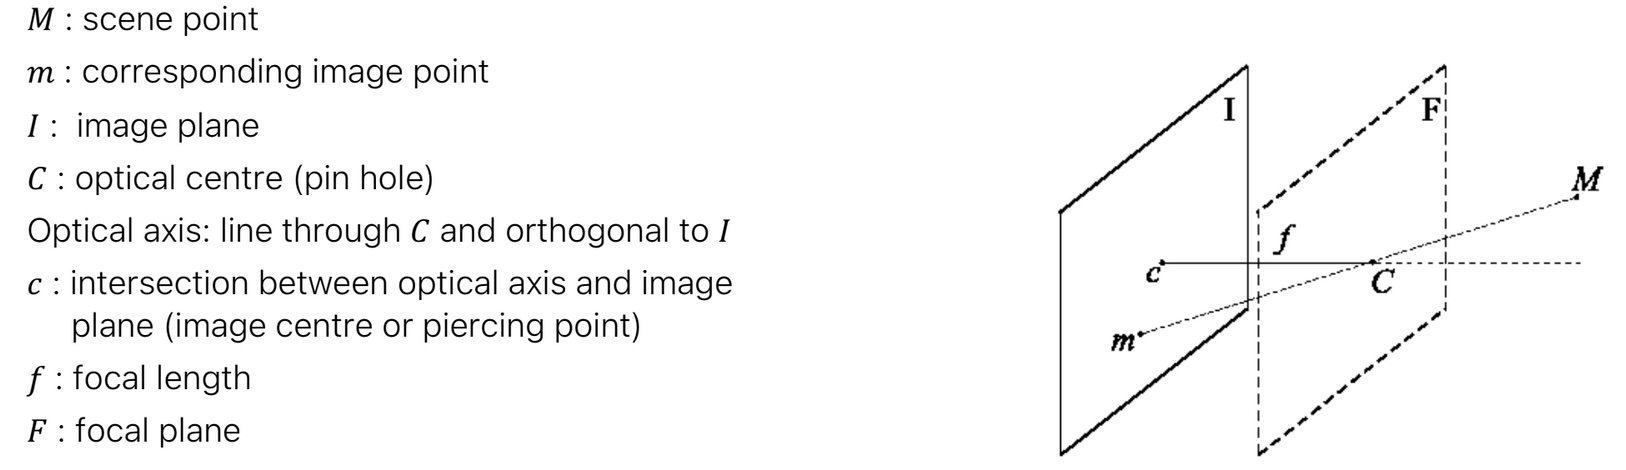
\includegraphics[width=0.9\linewidth]{./img/perspective_projection.jpg}
  \caption{perspective projection}
  % \label{}
\end{figure}

Which, by writing the poitns as vectors and the plane's coordinates becomes:

\begin{figure}[htbp]
  \centering
  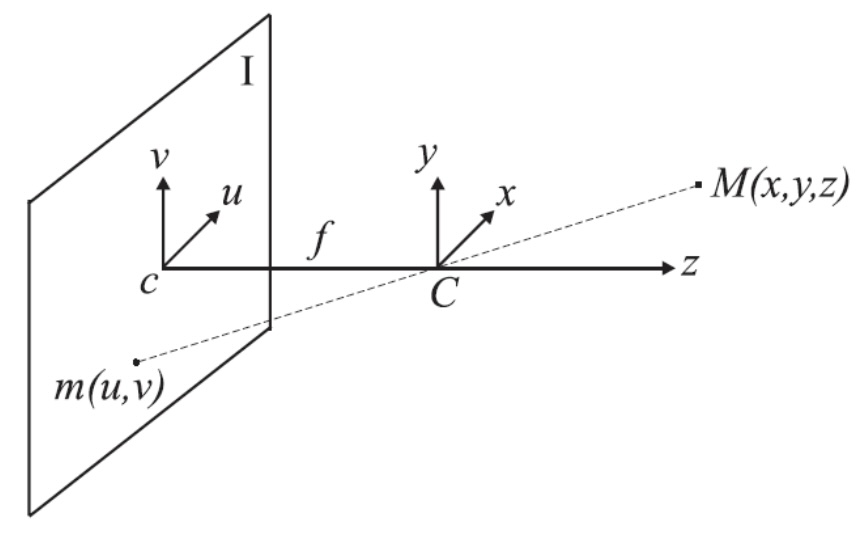
\includegraphics[width=0.45\linewidth]{./img/perspective_projection_axis.jpg}
  \caption{geometric model of image formation}
  \label{fig:perspective_projection_axis}
\end{figure}

Given the reference frame in \ref{fig:perspective_projection_axis} 
\begin{itemize}
  \item $u$ is the horizontal axis in the image plane.
  \item $v$ is the vertical axis in the image plane.
  \item $X$ and $Y$ are the respective axis in the 3D reference system. It's called the \textbf{camera reference system} because it is "attached" to the camera.
\end{itemize}

\textbf{For the perspective model these axis must be parallel}

The equations to map scene points into their corresponding image points are defined as:

$$\frac{u}{x} = -\frac{f}{z} \rightarrow u = -x\frac{f}{z} \quad\quad\quad \frac{v}{y} = - \frac{f}{z} \rightarrow v = -y\frac{f}{z}$$

The minus sign means the axis gets inverted (as we can see in the visualization, and it's what happens in the brain).
We can get rid of the sign, since the image plane can be though of as lying in front rather than behind the optical centre.

Image coordinates are a scaled version of scene coordinates (function of depth), this means that if the distance becomes bigger the object gets smaller.
When z increases, since it's at the denominator in both the equations the terms gets smaller (object gets smaller).
\textbf{The larger the focal length the bigger the object is in the image (and viceversa)}.

As we previously said, the image formation process deals with mapping a 3D space onto a 2D space, and so to a loss of information.
A given scene point is mapped into an image point, but an image point is mapped onto a 3D line.
For an image point we can only state that its corresponding scene point lays on al ine but cannot disambiguate a specific 3D point along such a line.

\subsubsection{Stereo images}

The solution is to use multiple images (at least two) to create stereo vision.
The human visual system is a stereo vision system.
Given correspondences, 3D information can be recovered easily by triangulation.
We can use two cameras, or two cameras and an infrared sensor to project guides to align the images.

For standard stereo geometry there are some assumptions we have to make:
\begin{itemize}
  \item The cameras have parallel $(x,y,z)$ axes.
  \item The image planes of both cameras are coplanar and aligned.
  \item Both cameras have identical focal lengths.
\end{itemize}

Based on this, the transformation between the two reference frames is just a translation, usually horizontal.
For stereo vision is also really important to \textbf{sense two images at the very same moment}.

The cameras are displaced at a given quantity $b$ called baseline.
The \textbf{disparity} is the difference between the horizontal coordinates in the left and right images.

\begin{figure}[htbp]
  \centering
  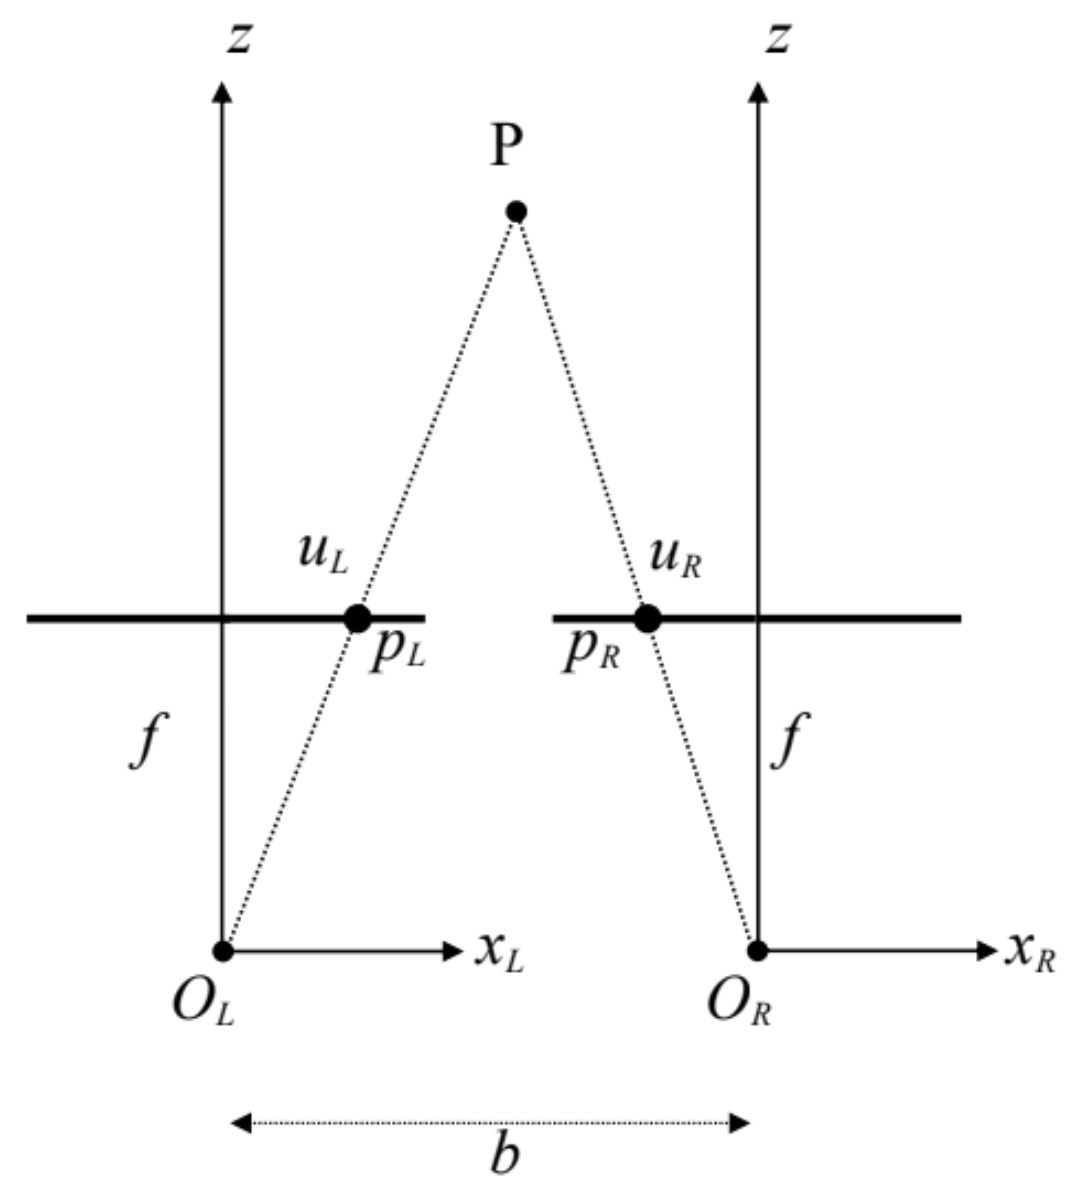
\includegraphics[width=0.45\linewidth]{./img/standard_stereo_geometry.jpg}
  \caption{standard stereo geometry}
  \label{fig:standard_stereo_geometry}
\end{figure}

The fundamental relationship in stereo vision is $z = b \cdot \frac{f}{d}$.
It's used to calculate the depth of a point in a scene from a pair of stereo images.

In standard stereo geometry since we are given just two 2D images there is no info about the correspondence between two points in the two images.
We can recall that the camera have parallel axes, and so we know that we can search for the correspondence alogn the horizontal lines.
This task is called stereo matching.

\subsubsection{Stereo correspondence}
Given a point in one image find it in the other image which is the projection of the same 3D point.
Such image points are called corresponding points.
\textbf{Points farther away have a smaller disparity, while close poitns have a larger display}

\begin{figure}[htbp]
  \centering
  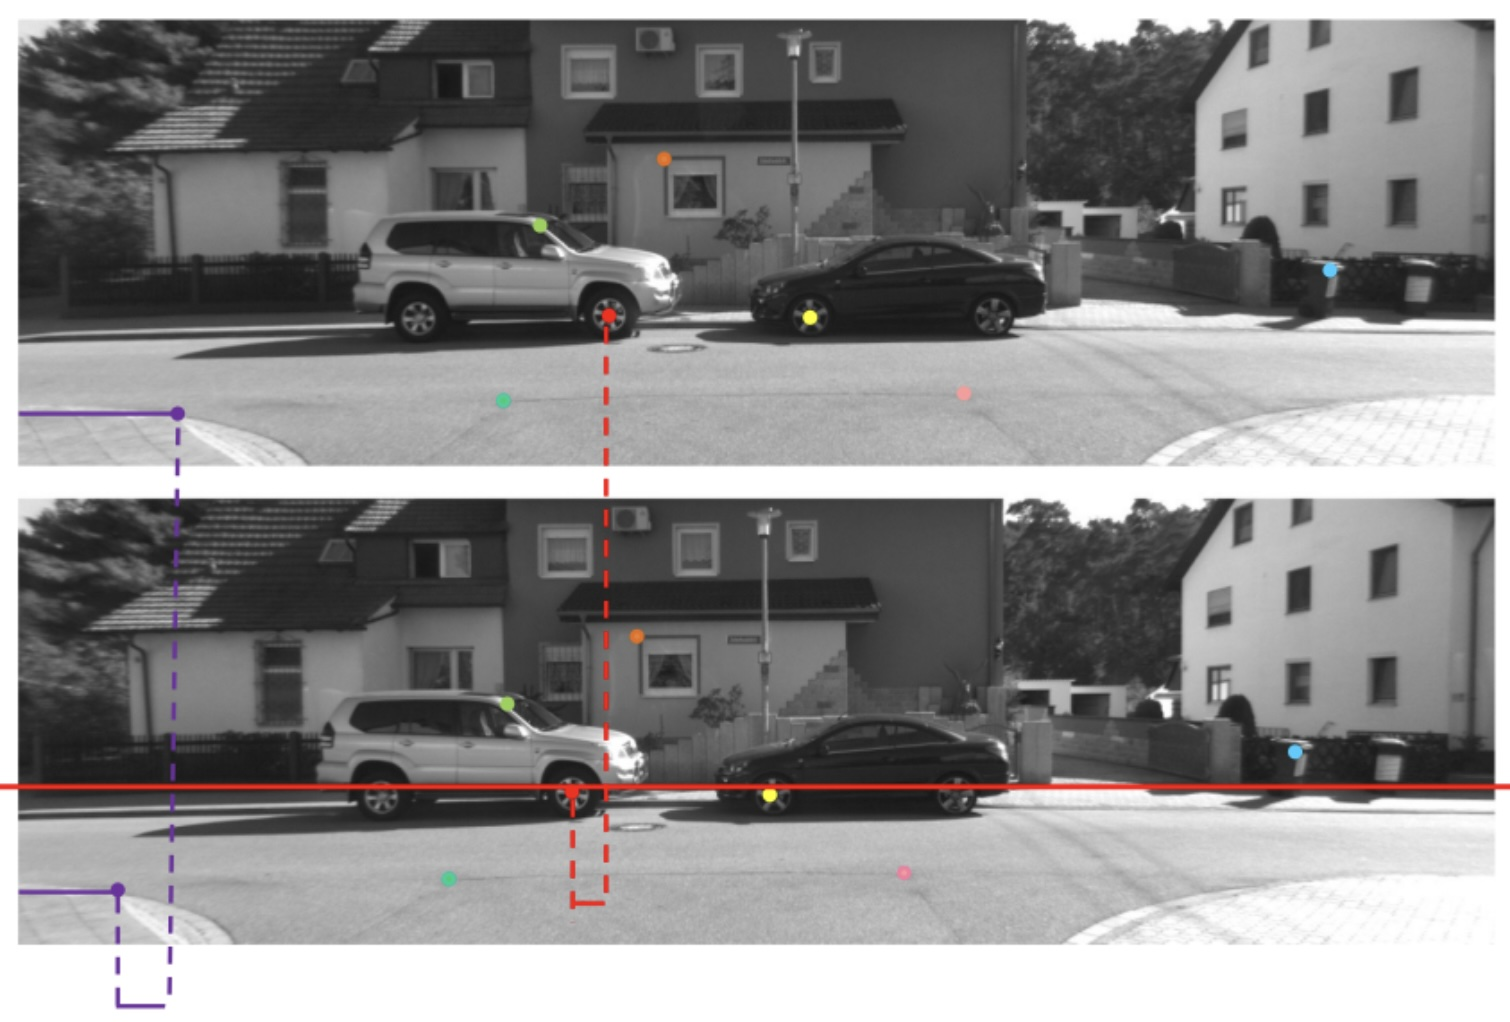
\includegraphics[width=0.65\linewidth]{./img/stereo_correspondence.jpg}
  \caption{Corresponding points look similar in the two images}
  \label{fig:stereo_correspondence}
\end{figure}

The image of a 3D line segment of length $L$ lying in a plane parallel to the image plane at distance $z$ from the optical centre will exhibit a length given by:
$$l = L \frac{f}{z}$$
This relationship is more complicated for an arbitrarily oriented 3D segment, as its position and orientation need to be accounted for as well.
For a \textbf{given position and orientation, length always shrinks alongside distance}.

Perspective projection maps 3D lines into image lines.
\textbf{Parallelism between 3D lines is not preserved} (except for lines parallel to the image plane).
This is the reason why if we look at a really long road into the distance we have the perception that the road becomes thinner, and the lines of the road intersect in the distance.
The images of parallel 3D lines intersect at a point, called \textbf{vanishing point}, which isn't necessarily within the image.

If the lines are parallel to the image plane they meet at infinity.

\subsubsection{Epipolar geometry}

What if the two cameras are no longer aligned? Do we need to search through the whole image?
We can project the line related to point $P_L$ in the right plane and search across that line.
The issue is that this projection can be computed only if the transformation between the two cameras is known (the relative mapping between the two cameras).

\begin{figure}[htbp]
  \centering
  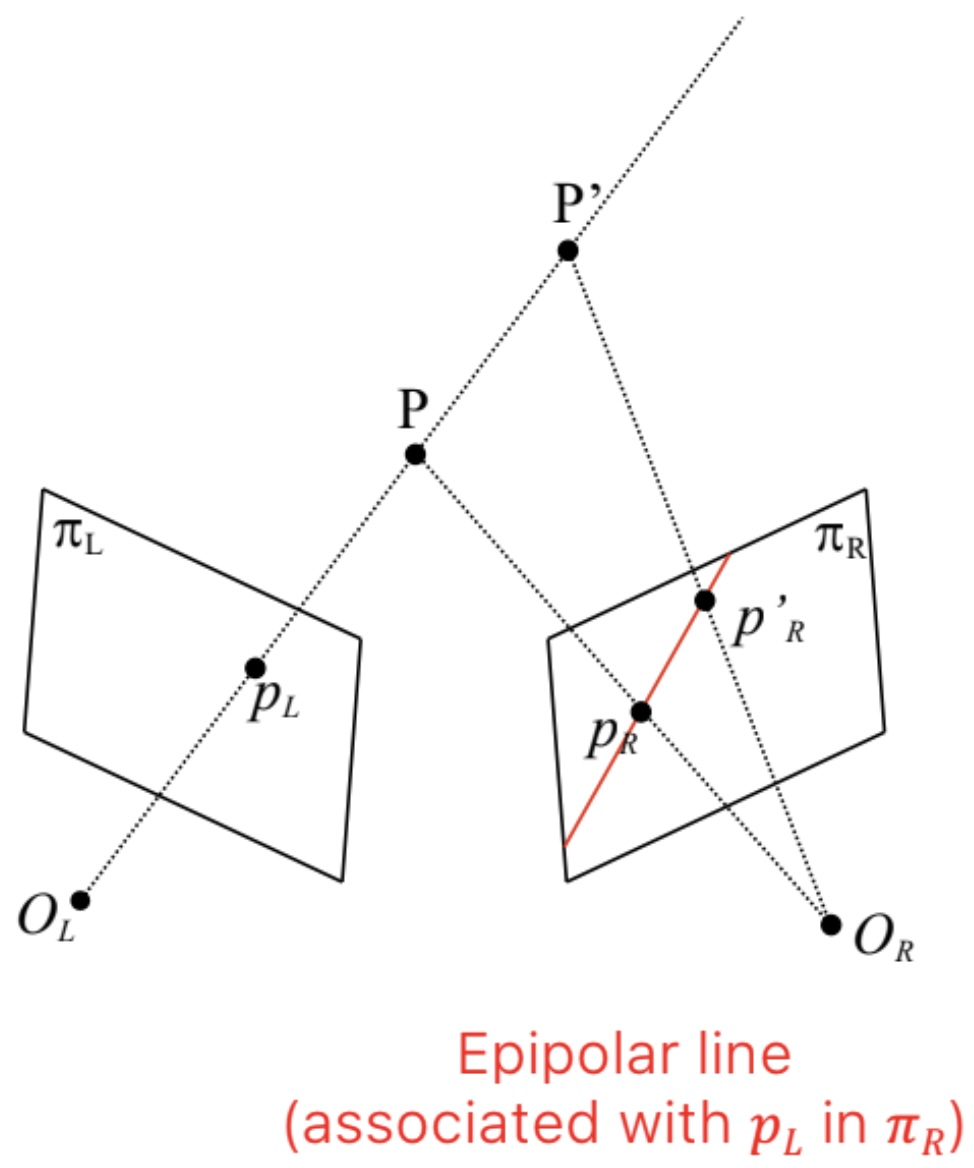
\includegraphics[width=0.45\linewidth]{./img/epipolar_line.jpg}
  \caption{Epipolar line}
  \label{fig:epipolar_line}
\end{figure}

It is almost impossible to build a stereo rig which is perfectly aligned horizontally.
Searching through oblique epipolar lines is awkward, and computationally is less efficient.
What people do in practice is to convert epipolar geometry to standard geometry with rectification/warping.
We warp the images as if they were acquired through a standard geometry, then we can compute and applyto both images a transformation known as rectification.

\subsubsection{Depth of Field (DOF)}

A scene point is on focus when all its light rays, gathered by the camera, hit the image plane at the same point.
In a pinhole device this happens to all scene points because of the very small size of the hole, so that the camera features an infinite Depth of Field (DOF).

The drawback is that such a small aperture allows gathering a very limited amount of light.
The image is really sharp, but has a really low light.
If a point is projected onto a circle instead of a point (bigger pinhole) the image is not sharp (not on focus).
If we cannot gather through aperture we have to integrate through time, by using a longer exposure time.

\subsubsection{Lenses}

Lenses concentrate light, so we use them to gather more light from a scene point and focus it on a single image point.
This enables much smaller exposure times.
This way Depth Of Field is no longer infinite, and only points across a limited range of distances can be simultaneously on focus in a given image.


We will consider the approximate model known as thin lens equation, which is useful to graphically determine the position of a focused image point:
\begin{itemize}
  \item Rays parallel to the optical axis are deflected to pass through $F$.
  \item Rays through $C$ are undeflected.
\end{itemize}

\textbf{If the image is on focus}, the image formation process obeys to the perspective projection model:
\begin{itemize}
  \item The center of the lens is the optical center.
  \item The distance $v$ acts as the effective focal length of the projection.
\end{itemize}

\begin{figure}[htbp]
  \centering
  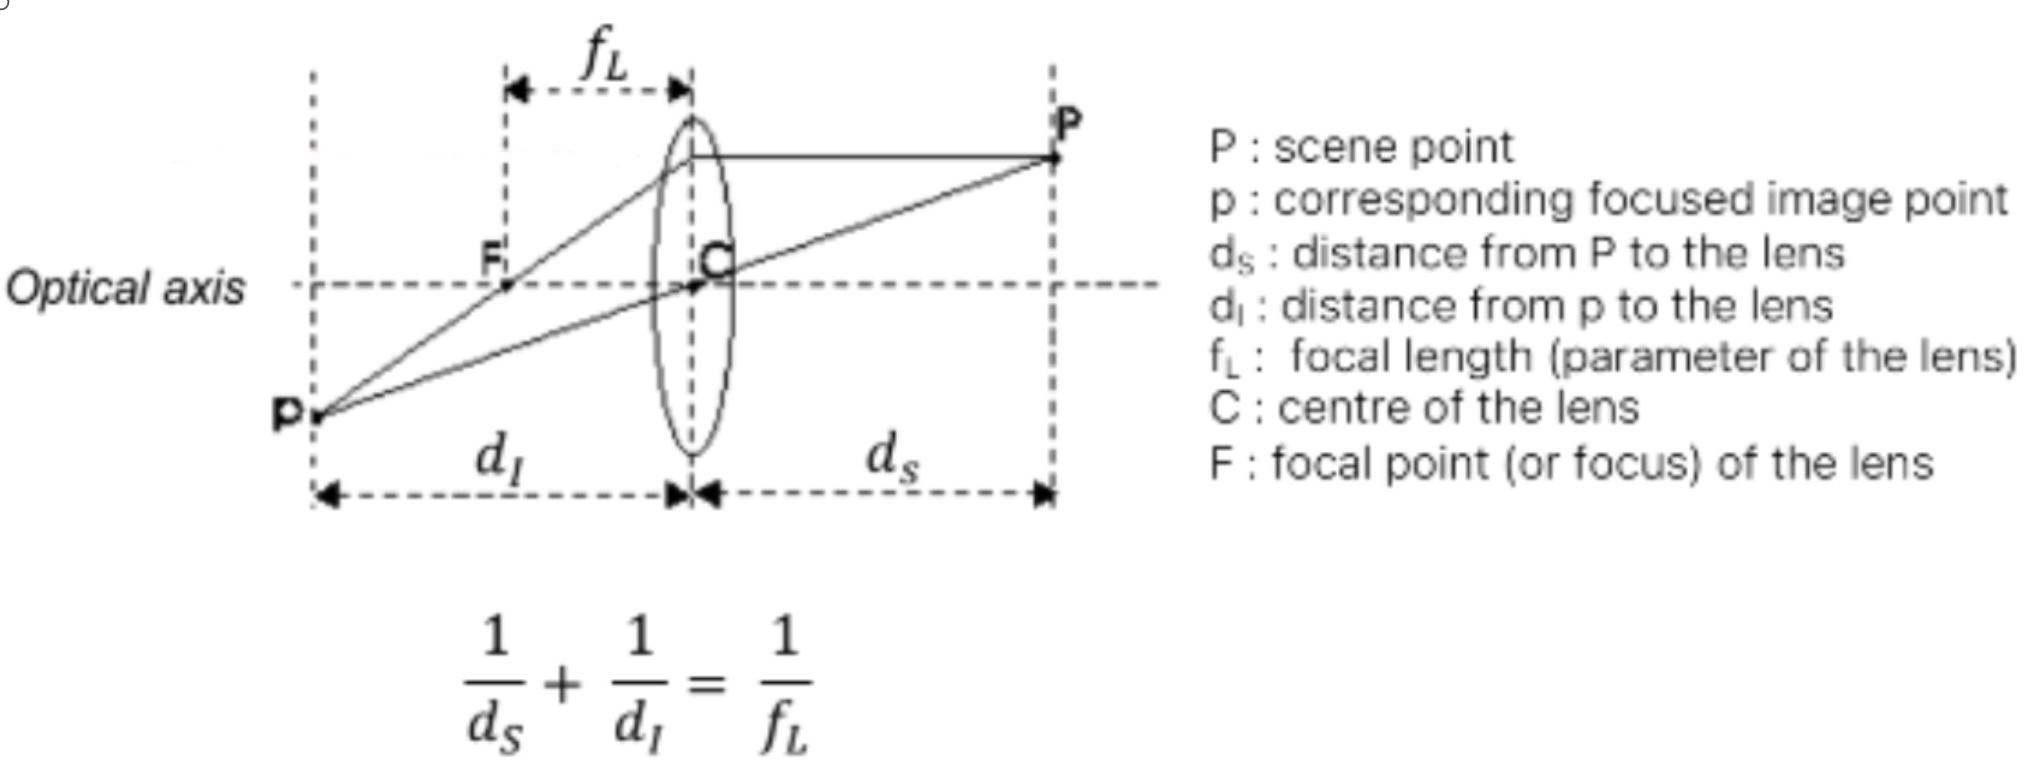
\includegraphics[width=0.7\linewidth]{./img/lens.jpg}
  \caption{Scheme of a lens}
  \label{fig:lens}
\end{figure}

Choosing the distance of the image plane determines the distance at which scene points appear on focus in the image.
Scene points in front and behind the focusing plane will result out-of-focus, thereby appearing in the image as circles, known as circles of confusion, or \textbf{blur circles}, rather than points.

The advantage of lenses is to have a small exposure time for capturing moving objects but we pay in terms of Depth Of Field.

\begin{figure}[htbp]
  \centering
  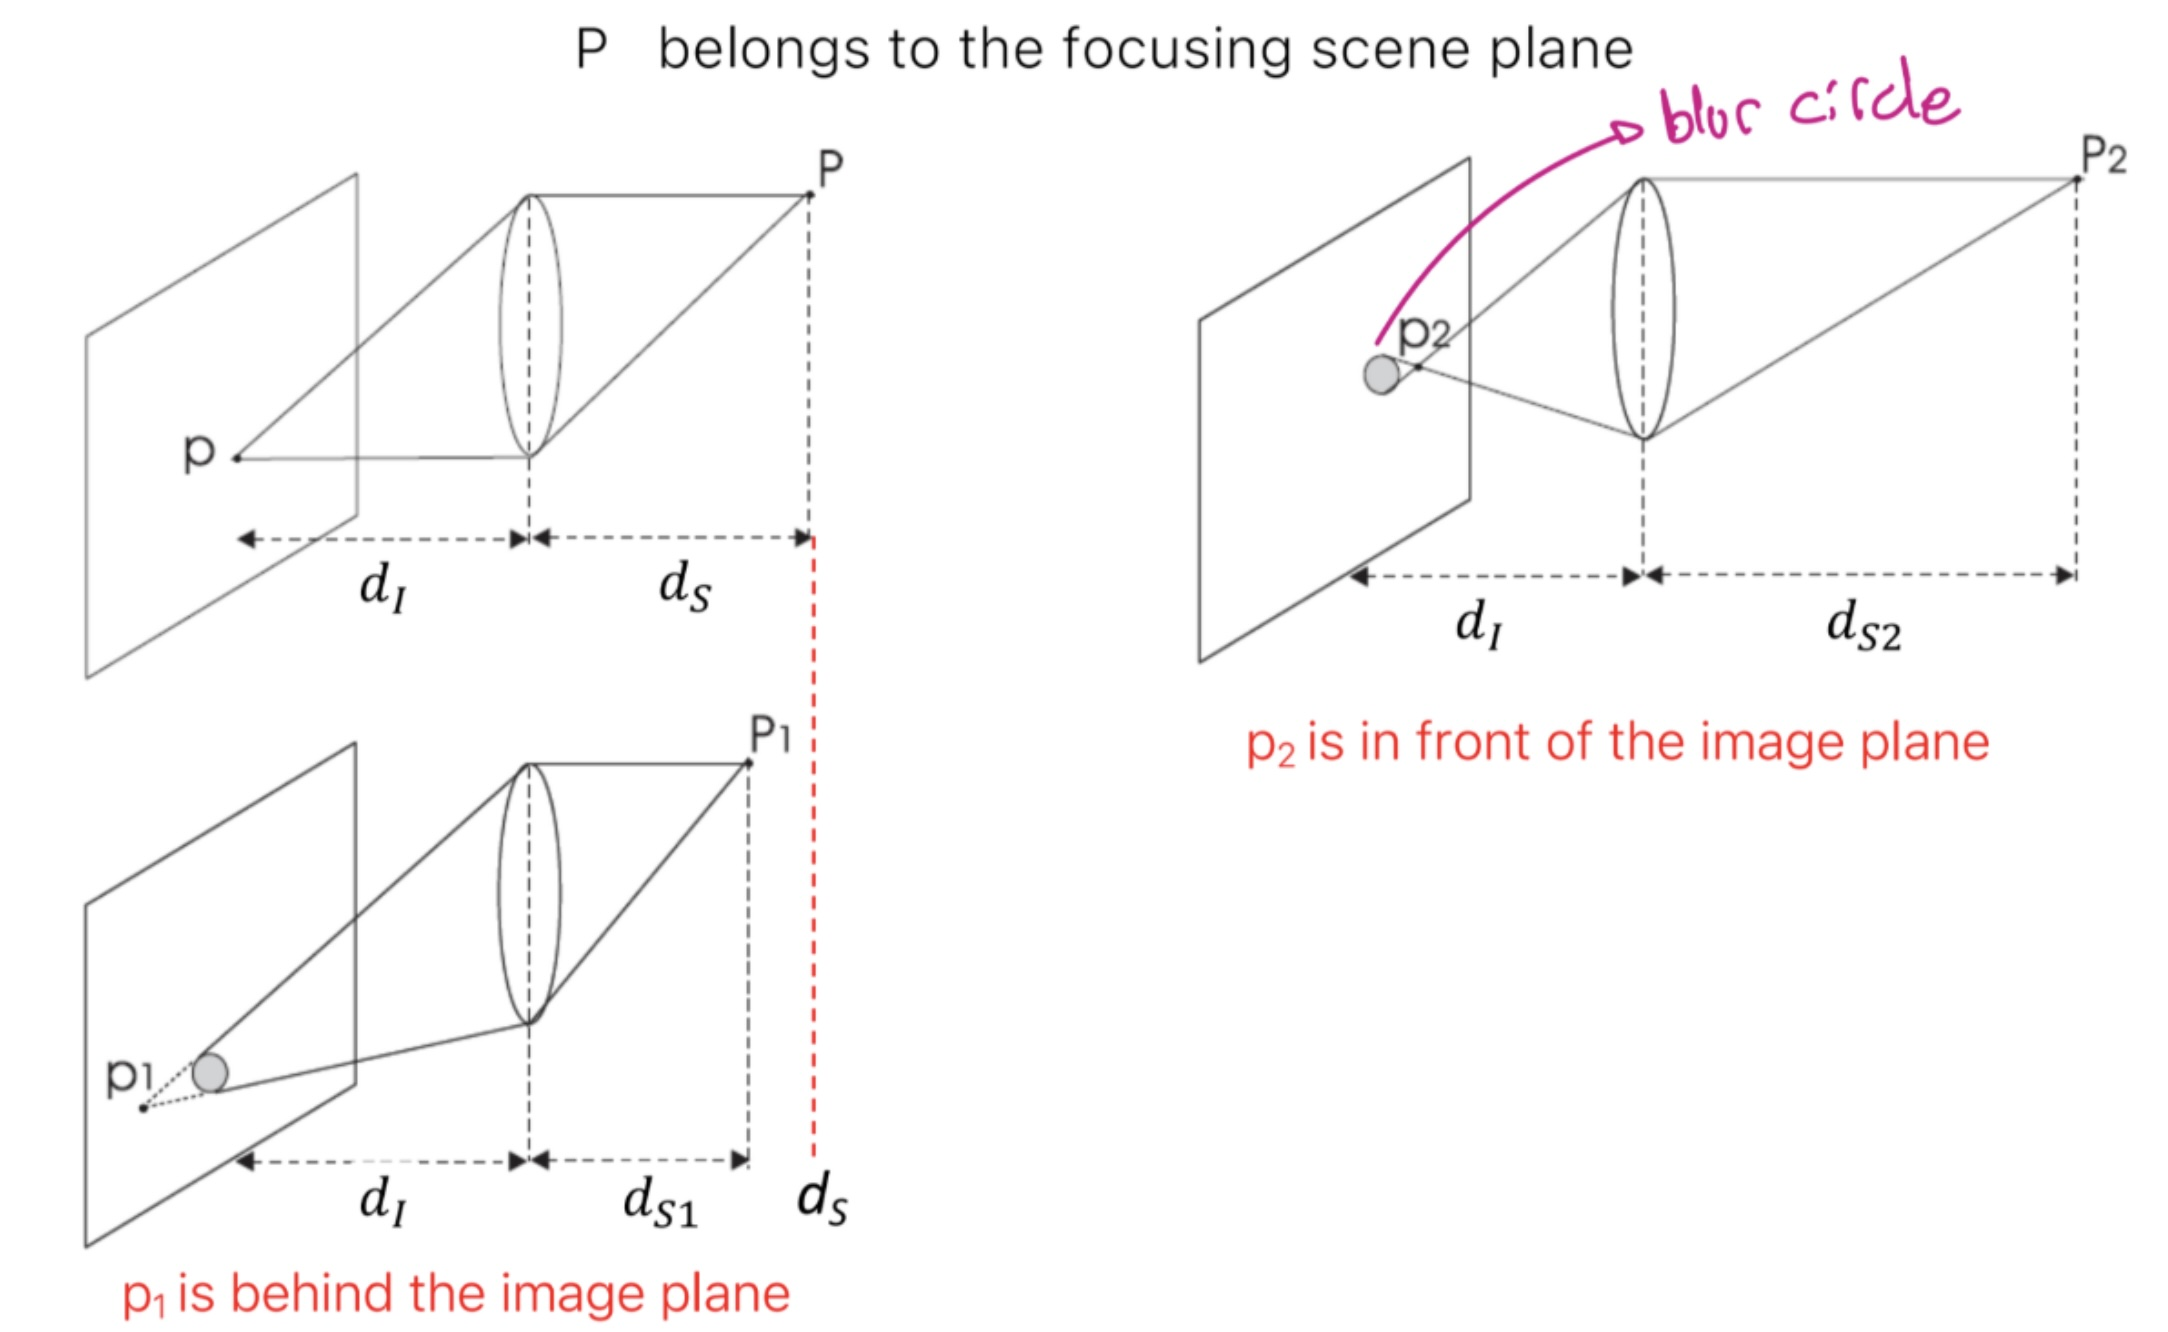
\includegraphics[width=0.7\linewidth]{./img/lens_focus.jpg}
  \caption{Lens focusing at various distances}
  \label{fig:lens_focus}
\end{figure}

\subsubsection{Diaphragm}

In theory, when imaging a scene through a thin lens, only the points at a certain distance can be on focus, all the others appear blurred into circles.
However, as long as the circles are smaller than the size of the photosensing elements (a single pixel), the image will still look on-focus.

\begin{figure}[htbp]
  \centering
  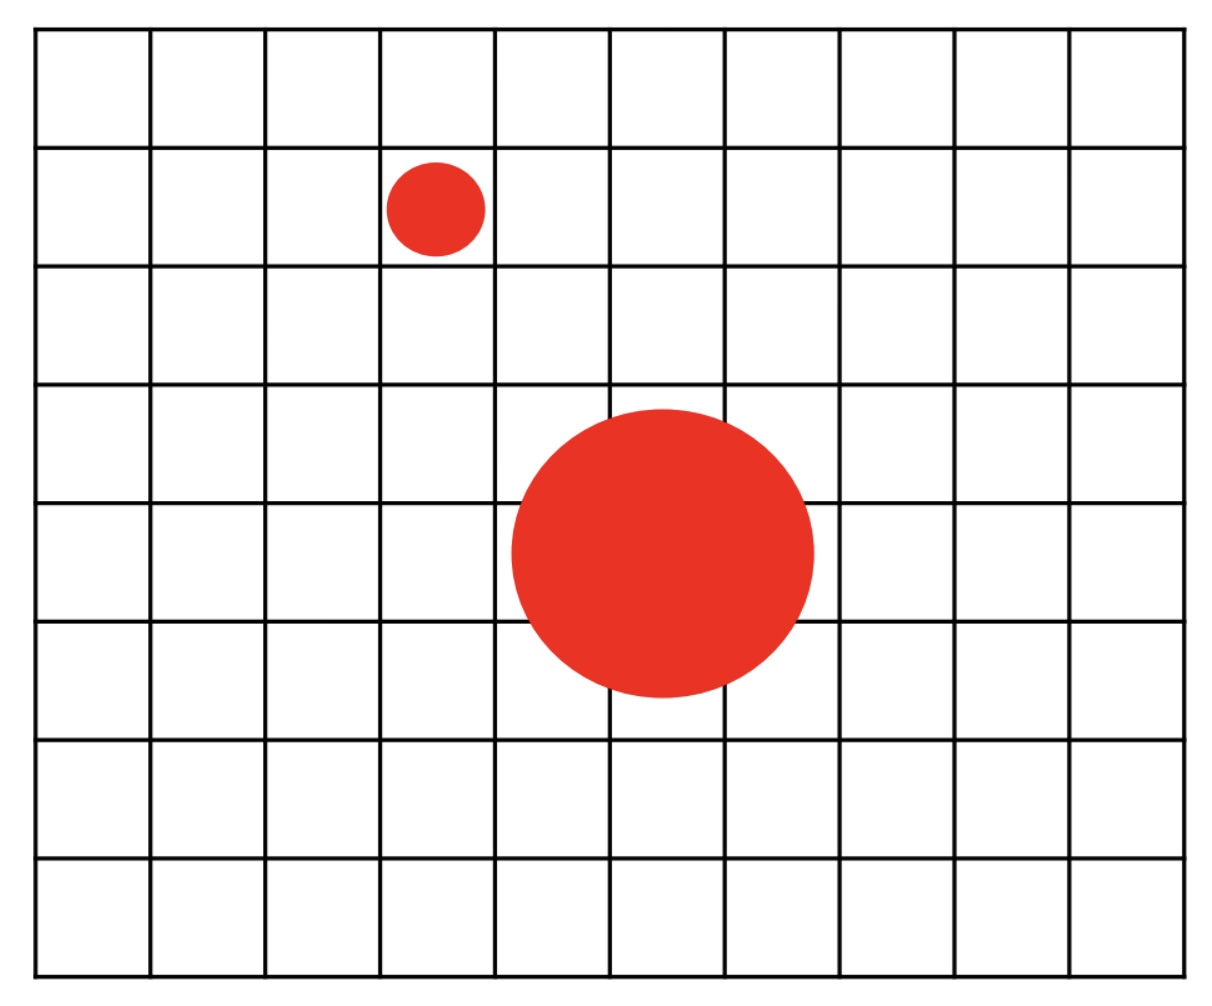
\includegraphics[width=0.55\linewidth]{./img/diaphragm.jpg}
  \caption{Blurring at pixel level}
  \label{fig:diaphragm}
\end{figure}

The range of distances across which the image appears on focus, due to blur circles being small enough, determines the Depth Of Field) of the imaging apparatus.
Cameras often deploy an adjustable diaphragm (iris) to control the amount of light gathered through the effective aperture of the lens.
\begin{itemize}
  \item Reduce aperture $\rightarrow$ less light $\rightarrow$ smaller blur circle
  \item More aperture $\rightarrow$ more light $\rightarrow$ larger blur circle.
  \item Close the diaphragm $\rightarrow$ increase depth of field $\rightarrow$ not enough light $\rightarrow$ increase exposure time $\rightarrow$ moving object $\rightarrow$ motion blur $\rightarrow$ still scenes.
\end{itemize}

\subsubsection{Focusing mechanism (manually changing depth of field)}
To focus on objects at diverse distances we need a amechanism that allows the lens (or the lens subsystem) to translate along the optical axis with respect to the fixed position of the image plane.

\begin{figure}[htbp]
  \centering
  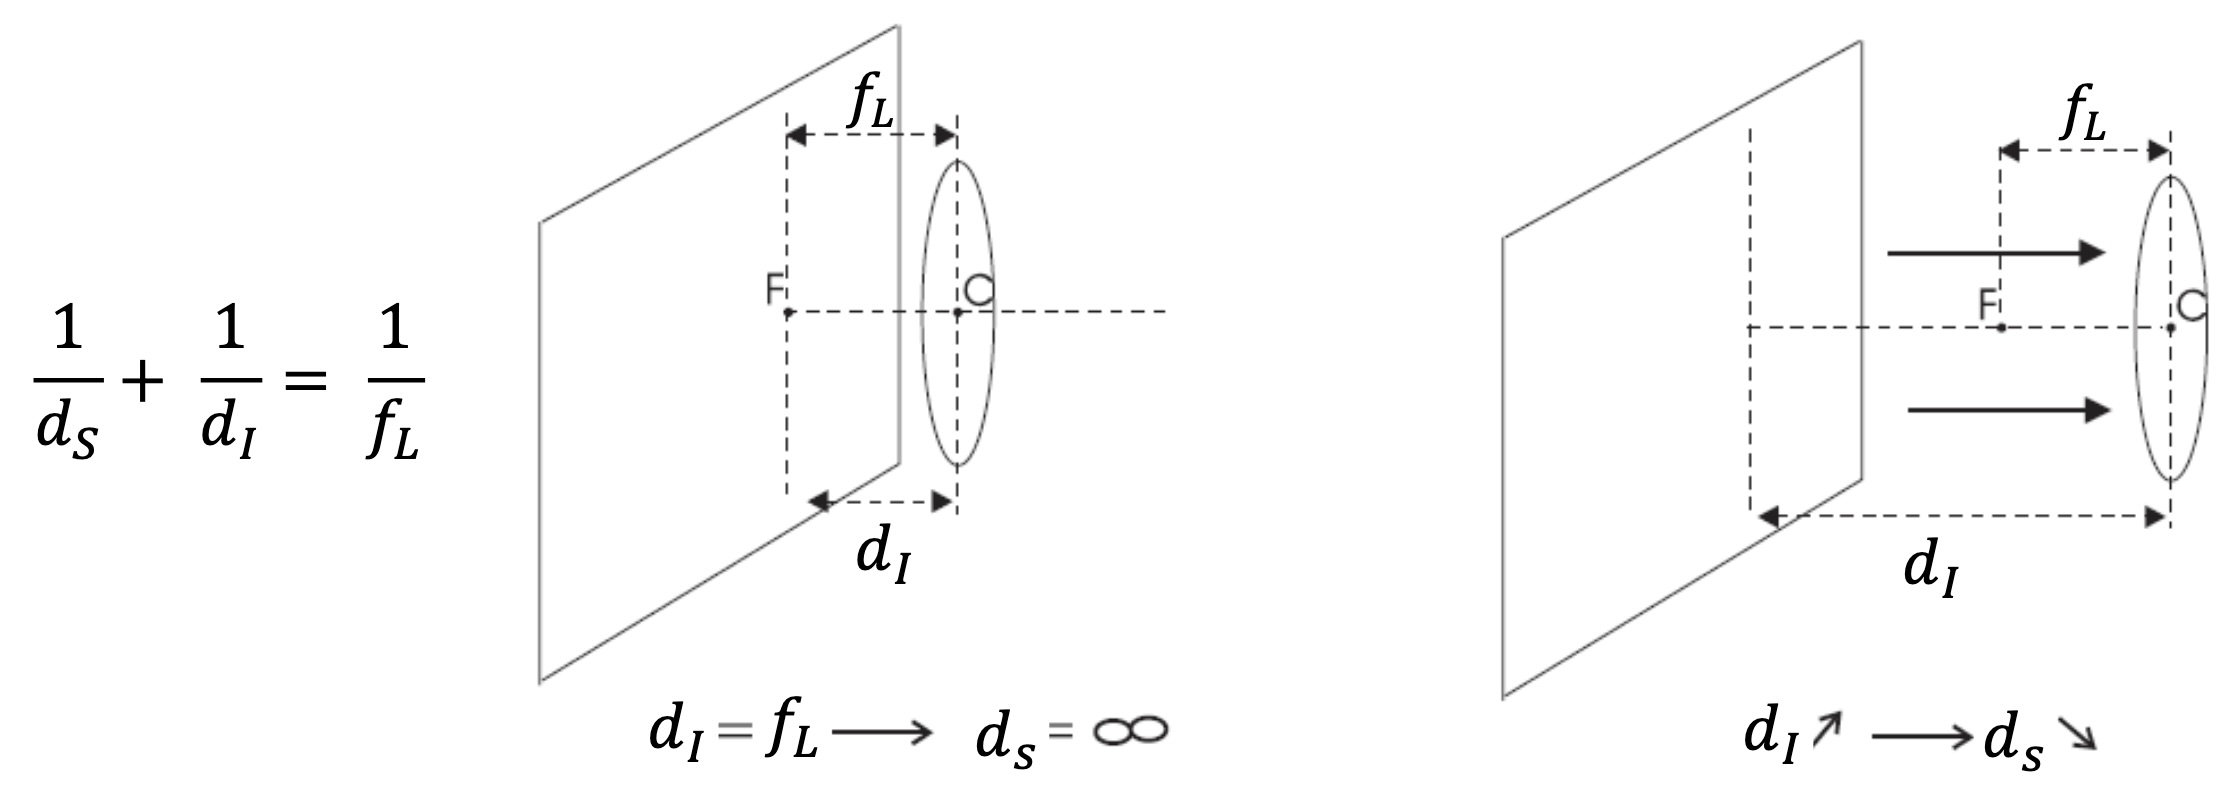
\includegraphics[width=0.7\linewidth]{./img/focusing_mechanism.jpg}
  \caption{Focusing mechanism}
  \label{fig:focusing_mechanism}
\end{figure}

At one end position ($d_I = f_L$) the camera is focused at infinity (objects at inifity are on sharp focus).
The focusing mechanism allows the lens to be translated farther away from the image plane up to a certain maximum value, which determines the minimum focusing distance.

\subsubsection{Image digitization}

How do we convert a continuous image to a discrete one which can be represented on a computer? 
The process can be divided in two steps: sampling and quanitzation.

\begin{figure}[htbp]
  \centering
  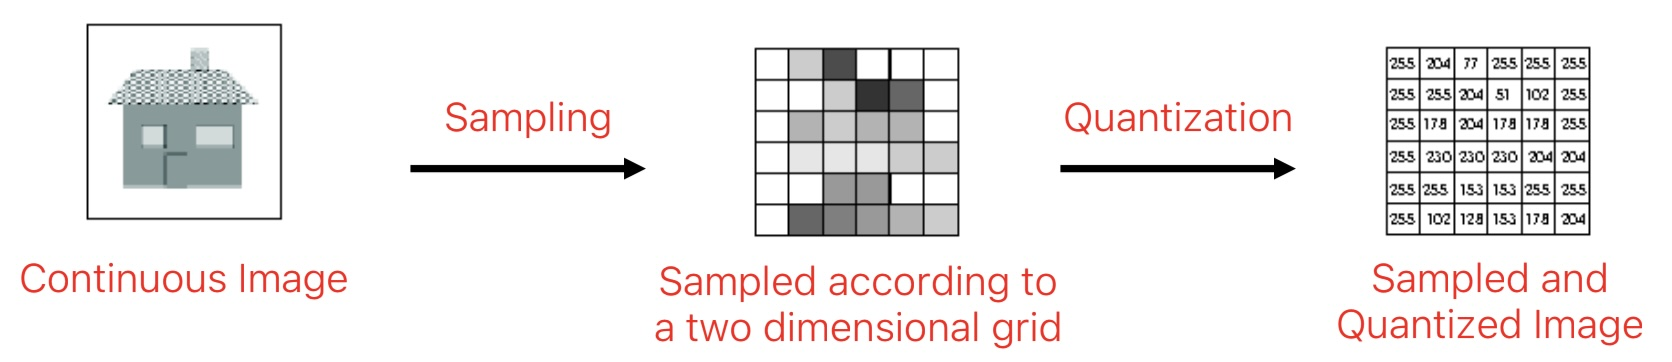
\includegraphics[width=0.55\linewidth]{./img/image_digitization.jpg}
  \caption{The two steps of the image digitization process}
  \label{fig:image_digitization}
\end{figure}

\begin{itemize}
  \item \textbf{Sampling}: the planar continuous image is sampled along both the horizontal and vertical directions to pick up a matrix of $n\times m$ samples known as pixels.
  \item \textbf{Quantization}: the continuous range of values associated with pixels is quantized into $l=2^m$ discrete levels known as gray-levels.
  $m$ is the number of bits used to represent a pixel, with the memory occupancy (in bits) of a gray-scale image given by $B = N \times M \times m$. Coloured digital images are typically represented within computers using 3 bytes per pixels. Both more pixels and more bits per pixel result in a higher quality image.
\end{itemize}

The more bits we spend for its representation, the higher the quality of the digital image (becomes a closer approximation to the ideal continuous image).
This applies both to sampling and quantization.

\subsubsection{Camera sensors}

The sensor is a matrix of photodetectors.
During exposure time, each detector converts the incident light into a proportional electic charge.
The companion circuitry reads-out the charge to generate the output signal, which can be either digital or analog.
For digital cameras the sensor includes the necessary ADC circuitry.

Today, the two main sensor technologies are:
\begin{itemize}
  \item Charge Coupled Devices (CCD), where the sensor and circuit are separated.
  \item CMOS (Complementary Metal Oxide Semiconductor), where everything is on the same circuit.
\end{itemize}

CCD/CMOS sensors can't sense colors, so we place an array of optical filters in front of the photodetectors, to render each pixel sensitive to a specific range of wavelengths.

\subsubsection{SNR}

The intensity measured at a pixel under perfectly static conditions varies due to the presence of random noise.
The main noise sources are:
\begin{itemize}
  \item \textbf{Photon Shot Noise}: the number of photons collected during exposure time is not constant.
  \item \textbf{Electronic Circuitry Noise}: generated by the electronics.
  \item \textbf{Quantization Noise}: related to the ADC conversion.
  \item \textbf{Dark Current Noise}: random charge observed due to thermal excitement.
\end{itemize}

SNR can be expressed both in decibels and bits.

\subsubsection{Dynamic Range (DR)}
If the sensed amount of light is too small, the "true" signal cannot be distinguished from noise.
Given $E_{\text{min}}$: the minimum detectable irradiation, and $E_{\text{max}}$, the saturation irradiation.
The Dynamic Range (DR) of a sensor is defined as $DR = \frac{E_{\text{max}}}{E_{\text{min}}}$, and like the SNR, it is often specified in decibels or bits.

Like SNR, the higher the DR the better it is.
A higher DR corresponds to the ability of the sensor to simultaneously capture in one image both the dark and bright structures of the scene.

% lecture 2 part 2
\subsection{Image Filtering}

\subsubsection{Noise and image filters}

In computer vision we have to deal with noise.
Noise is always different and more noticeable in uniform regions of the image.
The simplest thing to reduce noise is to output the average of the pixel color over time, to get \textbf{almost} the ideal noiseless value.
$$O(p) = \frac{1}{T} \sum_{t=1}^{T} I_k(p) = \frac{1}{T} \sum_{t=1}^{T}(\tilde{I}(p) + n_t(p))$$

This technique works well on still images.

\begin{figure}[htbp]
  \centering
  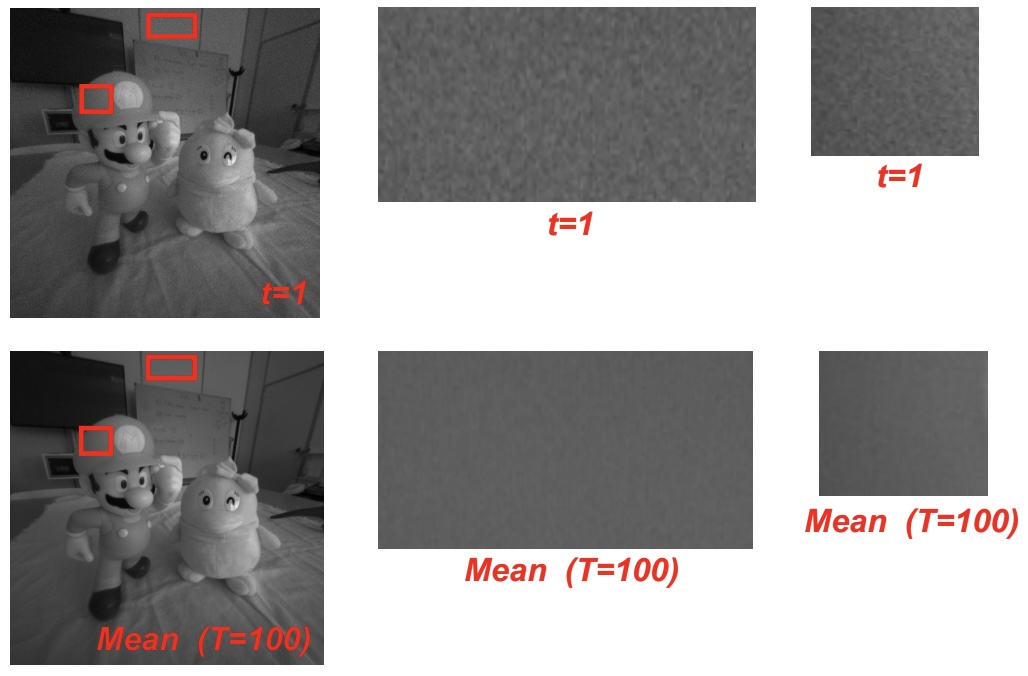
\includegraphics[width=0.7\linewidth]{./img/denoising_simple.jpg}
  \caption{Simple denoising}
  \label{fig:denoising_simple}
\end{figure}

If we are given a simple image, we may compute a mean across neighbouring pixels, like a spatial rather than temporal mean.
The size of the square of the neighbouring pixels is a tradeoff.

This is a very basic denoising filter.

Image filters are image processing operators that compute the new intensity (colour) of a pixel, $p$, based on the intensities (colours) of those belonging to a neighbourhood (support) of $p$.

\subsubsection{Convolution}

An important sub-class of filters is given by \textbf{Linear} and \textbf{Translation-Equivariant (LTE)} operators.

The application of filters in image processing consists in a 2D convolution between the input image and the impulse response function of the LTE operator.

LTE operators are used as feature extractors in Convolutional Neural Networks (CNNs).

Given an input 2D signal $i(x,y)$, a 2D operator $T{i(x,y)}$ is said to be linear if and only if
$$ T{\alpha i_1(x,y) + \beta i_2(x,y)} = \alpha o_1(x,y) + \beta o_2(x,y) $$ with $o_1 = T{i_1}$ and $o_2 = T{i_2}$ and $\alpha, \beta$ are two constants.
The operator is said to be \textbf{translation-equivariant} if and only if: $T{i(x-x_0, y-y_0)} = o(x-x_0, y-y_0)$

If the operator is LTE, the output signal is given by the \textbf{convolution} between the input signal and the impulse response (point spread function) $h(x,y) = T{\delta (x,y)}$.

$$o(x,y) = i(x,y) * h(x,y) = T{i(x,y)}$$

$$i(x,y) * h(x,y) = \int_{-\infty}^{\infty} \int_{-\infty}^{\infty} i(\alpha, \beta) h(x-\alpha, y-\beta) \, d\alpha  d\beta $$

\begin{figure}[htbp]
  \centering
  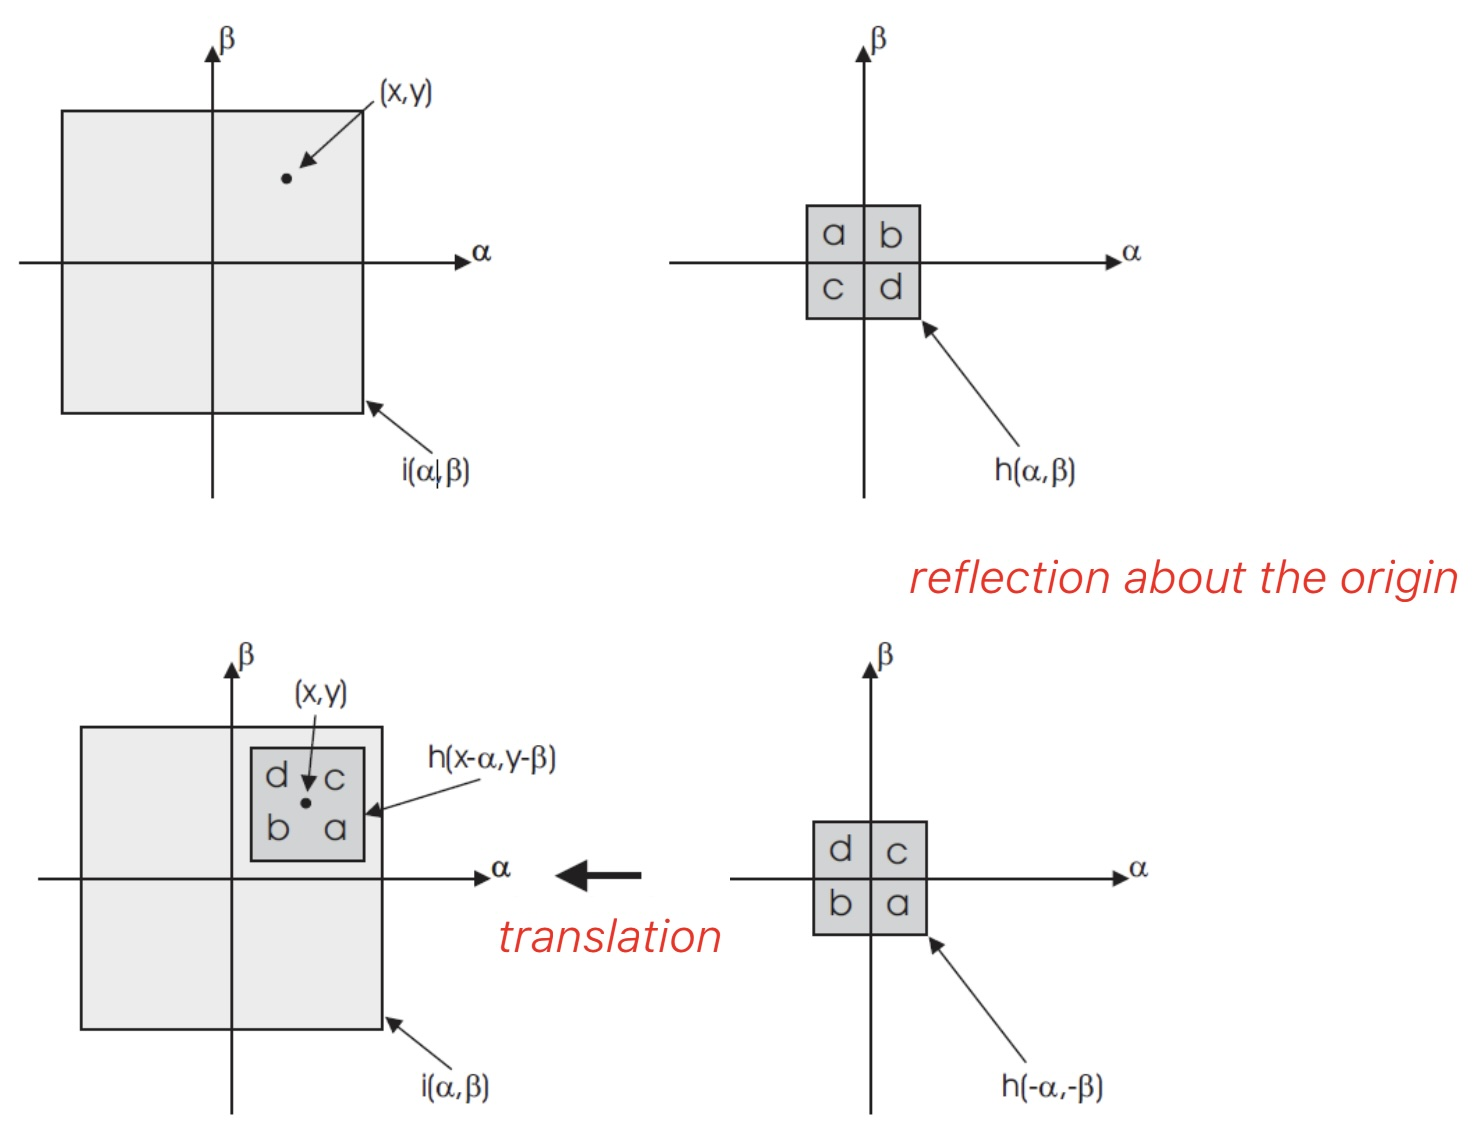
\includegraphics[width=0.7\linewidth]{./img/graphical_convolution.jpg}
  \caption{A graphical view of convolution}
  \label{fig:graphical_convolution}
\end{figure}

Convolutions have some useful properties:
\begin{itemize}
  \item \textbf{Associative property}: $f * (g * h) = (f*g)*h$ (useful because we can decompose kernels and obtain faster operations).
  \item \textbf{Commutative property}: $f*g = g*f$.
  \item \textbf{Distributive property}: $f*(g+h) = f*g + f*h$.
  \item \textbf{Convolution commutes with differentiation}: $(f*g)' = f'*g = f*g'$.
\end{itemize}

The correlation of signal $i(x,y)$  with respect to signal $h(x,y)$ is defined as:
$$i(x,y) \circ h(x,y) = \int_{-\infty}^{\infty} \int_{-\infty}^{\infty} i(\alpha, \beta) h(x-\alpha, y-\beta) \, d\alpha  d\beta $$

Correlation is not commutative, unlike the convolution.

\subsubsection{Discrete convolution}

Normal convolution is useful for signal theory, but we want to have a discrete convolution, where we use summations instead of integrals.
The four convolution properties highlighted for the convolution hold for the discrete one too.

\subsubsection{Practical implementation}
CNNs learn flipped kernels.
In image processing both the the input image and the kernel are stored into matrices of given finite sizes, with the image being much larger than the kernel.
Conceptually, to obtain the output image we need to slide the kernel across the whole input image and compute the convolution at each pixel.

We have an issue on borders, since the kernel "goes out" of the matrix of the image.
We have two main options to solve this issue:
\begin{itemize}
  \item \verb|CROP|: common in image processing.
  \item \verb|PAD|: preferred in CNNs. We can do zero-padding, replicate the first pixel many times, reflect the first $k$ pixels (half of the kernel)...
\end{itemize}

Without padding convolutions shrink the images.

\begin{figure}[htbp]
  \centering
  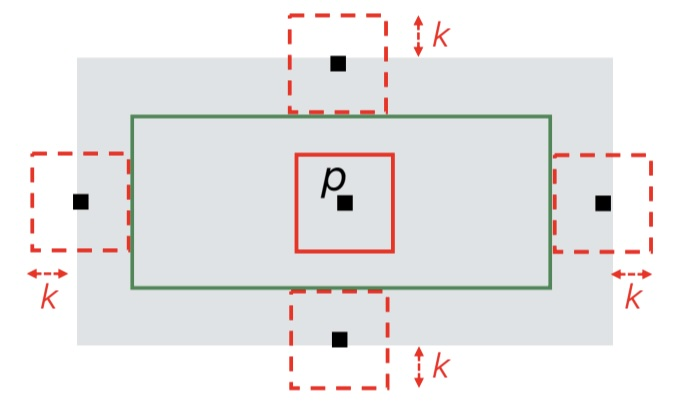
\includegraphics[width=0.7\linewidth]{./img/convolution_visualization.jpg}
  \caption{Issues with convolutions}
  \label{fig:convolution_visualization}
\end{figure}

\subsubsection{Mean filter}

Mean filtering is the simplest and fastest way to denoise an image.
It consists in replacing each pixel intensity by the average intensity overa chosen neighbourhood.
According to signal processing theory, the Mean Filter carries out a low-pass filtering operation, which in image processing is also referred to as image smoothing.
Smoothing is often aimed at image denoising, but sometimes is used to cancel out small-size unwanted details that might hinder the image analysis task.
Linear filtering reduces noise but blurs the image, so we lose sharpness.

\subsubsection{Gaussian filter}



% lecture 3 
\section{Advanced Topics in Deep Learning for Computer Vision}

\end{document}
